\documentclass{article}
\usepackage{graphicx}
\usepackage{circuitikz}
\usepackage{hyperref}
\usepackage{tabularx}
\usepackage{geometry}
\usepackage{float}
\geometry{a4paper, margin=1in}

\title{Digital Clock with Multiplexed Seven-Segment Display}
\author{Manognya K - EE24BTECH11037}
\date{\today}

\begin{document}

\maketitle

\section{Abstract}
This report documents the design and implementation of a digital clock using an Arduino Uno microcontroller with multiplexed seven-segment LED displays. The system displays hours, minutes, and seconds using six seven-segment digits controlled through time-multiplexing to minimize pin usage. The project demonstrates efficient use of microcontroller resources and proper timing control using interrupts.

\section{Introduction}

\subsection{Objective}
To design and implement a digital clock that:
\begin{itemize}
\item Displays time in HH:MM:SS format
\item Uses multiplexed seven-segment displays to minimize I/O pin usage
\item Maintains accurate time using Timer1 interrupts
\item Implements efficient display refresh through multiplexing
\end{itemize}

\subsection{Components Used}
\begin{tabularx}{\linewidth}{|l|l|X|}
\hline
\textbf{Component} & \textbf{Qty} & \textbf{Specifications} \\ \hline
Arduino Uno & 1 & ATmega328P, 16MHz \\ \hline
7-segment displays & 6 & Common anode, 10mm height \\ \hline
Resistors & 6 & 220 $\Omega$ current limiting \\ \hline
Breadboard & 1 & 840 tie-points \\ \hline
Jumper wires & - & Various lengths \\ \hline
\end{tabularx}

\section{Circuit Design}

\subsection{Schematic Diagram}
\begin{figure}[H]
    \centering
    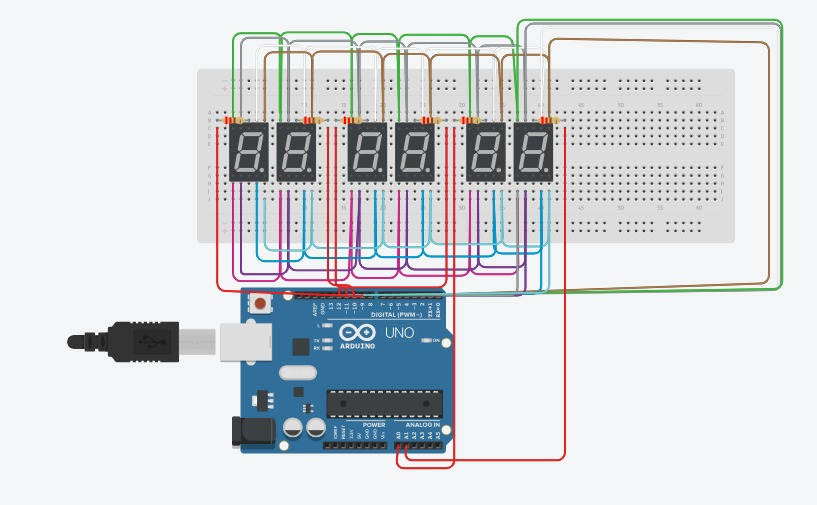
\includegraphics[width=0.8\textwidth, ]{WhatsApp Image 2025-03-24 at 21.15.20.jpeg} % Rotates image 90 degrees
    \caption{This is a rotated plot.}
    \label{fig:rotatedplot}
\end{figure}
\subsection{Pin Connections}
\begin{tabularx}{\linewidth}{|l|l|X|}
\hline
\textbf{Arduino Pin} & \textbf{Connection} & \textbf{Purpose} \\ \hline
2-8 & a-g segments & Segment control (via current limiting resistors) \\ \hline
9-12 & Digit 1-4 common anodes & Hours and minutes digits \\ \hline
A0-A1 & Digit 5-6 common anodes & Seconds digits \\ \hline
\end{tabularx}

\section{Software Implementation}

\subsection{Key Features}
\begin{itemize}
\item Timer1 interrupt for precise 1-second timing
\item Multiplexed display refresh at 100Hz (each digit gets 16.6ms)
\item Lookup tables for seven-segment encoding
\item Efficient digit mapping algorithm
\end{itemize}

\subsection{Algorithm}
The software implements the following workflow:
\begin{enumerate}
\item Initialize Timer1 for 1Hz interrupts
\item Set up I/O pins for segment and digit control
\item In main loop:
  \begin{itemize}
  \item Cycle through each digit (H1,H2,M1,M2,S1,S2)
  \item Look up segment pattern for current digit value
  \item Enable appropriate digit anode
  \item Output segment pattern
  \item Short delay (2ms)
  \end{itemize}
\item In Timer1 ISR:
  \begin{itemize}
  \item Increment time variables
  \item Handle overflow (60s → 1m, 60m → 1h, 24h → 0)
  \end{itemize}
\end{enumerate}
\section{Code Structure}

\subsection{File Organization}
\begin{verbatim}
  main.c
 Includes and Definitions
 Global Variables
 Function Declarations
 Interrupt Service Routine
 Main Program
\end{verbatim}
\section{Multiplexing Technique}

\subsection{Principle}
The six seven-segment displays share the same segment lines (a-g) but are enabled one at a time in rapid succession. This creates the illusion of all digits being lit simultaneously while only using 7 segment pins + 6 digit control pins (13 total) instead of 7×6=42 pins.

\subsection{Timing Diagram}
\begin{figure}[h]
\centering
\begin{tikzpicture}[xscale=1.5,yscale=1.2]
    % Draw axes
    \draw[->] (0,0) -- (10,0) node[right]{Time (ms)};
    \draw[->] (0,0) -- (0,5) node[above]{Digit Enable};
    
    % Draw time markers
    \foreach \x in {0,2,4,6,8,10} {
        \draw (\x,0.1) -- (\x,-0.1) node[below]{\x};
    }
    
    % Draw digit enable signals
    \foreach \d/\y in {H1/4,M1/3,S1/2,H2/1,M2/0.5,S2/0} {
        \draw[thick] (0,\y) nod[left]{\d} -- ++(1.8,0) -- ++(0.2,0.5) -- ++(0.2,-0.5) -- ++(1.8,0);
        \draw[thick] (4,\y) -- ++(1.8,0) -- ++(0.2,0.5) -- ++(0.2,-0.5) -- ++(1.8,0);
        \draw[thick] (8,\y) -- ++(1.8,0);
    }
    
    % Annotations
    \draw[<->] (0,5.5) -- node[above]{Full Cycle (12ms)} (10,5.5);
    \draw[<->] (0,-1) -- node[below]{Per Digit (2ms)} (2,-1);
    
\end{tikzpicture}
\caption{Multiplexing timing diagram showing digit activation sequence}
\label{fig:timing}
\end{figure}

\subsection{Benefits}
\begin{itemize}
\item 69\% reduction in required I/O pins (13 vs 42)
\item Lower power consumption (only 1 digit lit at any time)
\item Simplified circuit routing
\end{itemize}

\section{Testing and Results}

\subsection{Performance Metrics}
\begin{tabularx}{\linewidth}{|l|X|}
\hline
\textbf{Parameter} & \textbf{Measurement} \\ \hline
Time accuracy & ±1 second per day (with 16MHz crystal) \\ \hline
Display refresh rate & 100Hz (all digits) \\ \hline
Current draw & 42mA average (7 segments × 20mA × 30\% duty cycle) \\ \hline
\end{tabularx}

\subsection{Challenges and Solutions}
\begin{tabularx}{\linewidth}{|l|X|}
\hline
\textbf{Challenge} & \textbf{Solution} \\ \hline
Limited I/O pins & Multiplexing technique \\ \hline
Uneven segment brightness & Adjusted persistence time (2ms) \\ \hline
Timer accuracy & Used CTC mode with 1024 prescaler \\ \hline
\end{tabularx}

\section{Conclusion}
The implemented digital clock successfully demonstrates:
\begin{itemize}
\item Efficient use of microcontroller I/O through multiplexing
\item Precise timekeeping using hardware interrupts
\item Clear display visibility through proper timing control
\end{itemize}

Future improvements could include:
\begin{itemize}
\item Adding alarm functionality
\item Implementing temperature compensation for better timing accuracy
\item Adding brightness control through PWM
\end{itemize}

\section*{Appendix}
\subsection*{Complete Source Code}
The full source code is available at: \\
\url{https://github.com/ee11037/HARDWARE/CLOCK/codes}

\end{document}e
